\documentclass{article}
% main document, called main.tex
\usepackage{tikz}
\usetikzlibrary{external}


\usetikzlibrary{positioning}

\usepackage{xcolor}% http://ctan.org/pkg/xcolor

\usepackage{color,soul}
\usetikzlibrary{calc}
\usetikzlibrary{shapes.geometric, arrows, arrows.meta}
\usepackage{varwidth}% http://ctan.org/pkg/varwidth
\usetikzlibrary{shadows,trees, mindmap}
\usetikzlibrary{matrix}
\usetikzlibrary{fit}
\colorlet{orangegreen}{green!10!orange!90!}
\definecolor{darkgreen}{rgb}{0, 0.5, 0} 

\tikzexternalize % activate!
\begin{document}

\footnotesize{
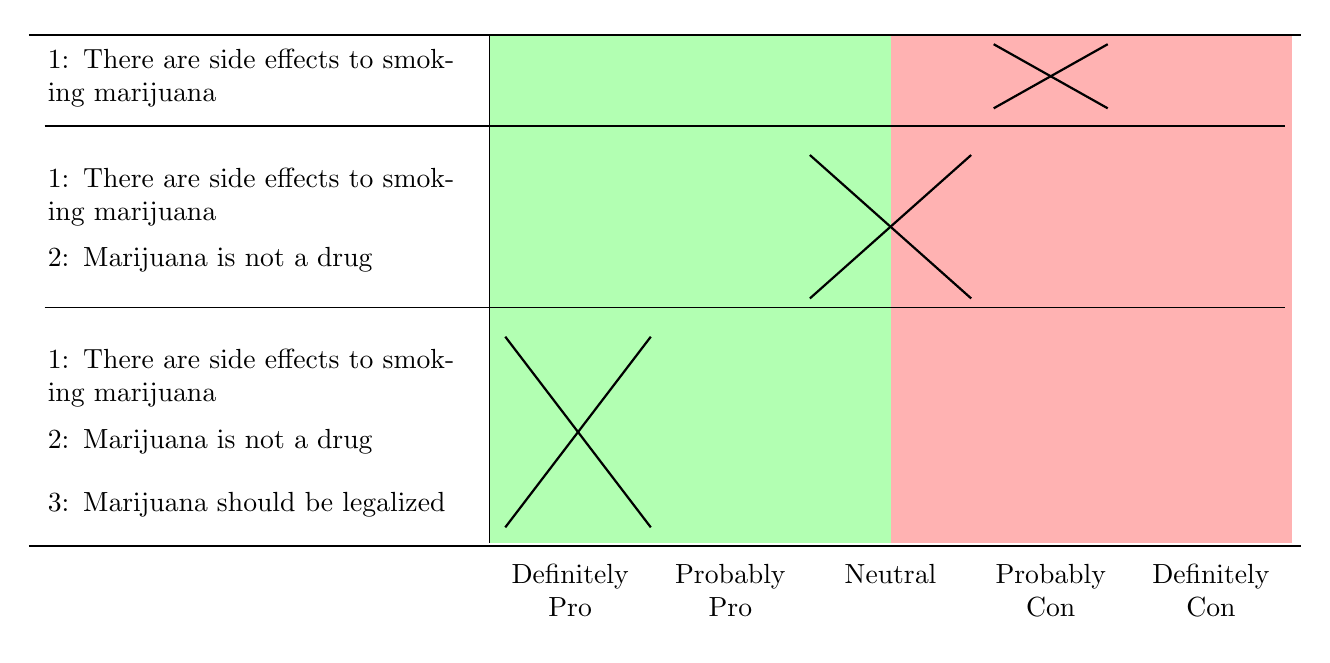
\begin{tikzpicture}[
lefttext/.style={rectangle, fill=white,
text width=5.5cm, text ragged, minimum height=0.5cm},
centertext/.style={rectangle, fill=white,
text width=1.8cm, text ragged, minimum height=0.8cm, align=center},
pro/.style={nodes={fill=green!30}},  
]
\node[matrix of nodes] (mymat) {
	\node [lefttext] (mymat-1-1) {1: There are side effects to smoking marijuana}; &
		\node[centertext] (topleft) {}; &
		\node[centertext] (grid-1-2){}; & 
		\node[centertext] (half-1) {}; &
		\node[centertext] (first) {}; &
		\node[centertext] (grid-1-5){}; & 
		\\[0.5cm]
\node [lefttext] (mymat-2-1) {1: There are side effects to smoking marijuana}; &
		\node[centertext] (grid-2-1){}; &
		\node[centertext] (grid-2-2){}; & 
		\node[centertext] (half-2) {}; &
		\node[centertext] (grid-2-4){}; &
		\node[centertext] (grid-2-5) {}; & 
		\\
		\node [lefttext] (mymat-3-1) {2: Marijuana is not a drug }; &
		\node[centertext] (grid-3-1){}; &
		\node[centertext] (grid-3-2){}; & 
		\node[centertext] (half-3) {}; &
		\node[centertext] (grid-3-4){}; &
		\node[centertext] (grid-3-5){}; & 
		\\[0.5cm]
		\node [lefttext] (mymat-4-1) {1: There are side effects to smoking marijuana}; &
		\node[centertext] (grid-4-1){}; &
		\node[centertext] (grid-4-2){}; & 
		\node[centertext] (half-4) {}; &
		\node[centertext] (grid-4-4){}; &
		\node[centertext] (grid-4-5){}; & 
		\\
		\node [lefttext] (mymat-5-1) {2: Marijuana is not a drug}; &
		\node[centertext] (third) {}; &
		\node[centertext] (grid-5-2) {}; & 
		\node[centertext] (half-5) {}; &
		\node[centertext] (grid-5-4) {}; &
		\node[centertext] (grid-5-5) {}; & 
		\\
		\node[lefttext] (mymat-6-1) {3: Marijuana should be legalized}; &
		\node[centertext] (bottomleft) {} ; &
		\node[centertext] (grid-6-2){}; & 
		\node[centertext] (half-6) {}; &
		\node[centertext] (grid-6-4) {}; &
		\node[centertext] (bottomright) {}; & 
		\\
		&
		\node [centertext] {Definitely Pro};  & 
		\node [centertext] {Probably Pro}; & 
		\node [centertext] {Neutral }; & 
		\node [centertext] (kre) {Probably Con}; & 
		\node [centertext] (bla) {Definitely Con}; \\
};

\draw[fill=green!30, draw=none] (topleft.north west)
rectangle ($(half-6.south west)!0.5!(half-6.south east)$);

\draw[fill=red!30, draw=none] ($(half-1.north west)!0.5!(half-1.north east)$)
rectangle (bottomright.south east);

% circles
% \draw ($(first.base) + (-0.2cm, 0.1cm)$) circle (0.2cm) node {\tiny{x}};
% \draw ($(half-3.base) +(-0.0005cm, 0.4cm) $) circle (0.2cm) node {\tiny{x}};
% \draw ($(third.base) + (0, 0)$) circle (0.2cm) node {\tiny{x}};

% x-marks the spot
%lower
\draw[thick] ($(bottomleft.south west) + (0.2cm, 0.2cm)$) -- 
($(grid-4-1.north east)$);
\draw[thick] ($(bottomleft.south east) + (0, 0.2cm)$) -- 
($(grid-4-1.north west) + (0.2cm, 0)$);

%middle
\draw[thick] (half-3.south west) -- 
(half-2.north east);
\draw[thick] (half-2.north west) -- 
(half-3.south east);

%upper
\draw[thick] ($(first.south west) + (0.3cm, -0.1cm)$) --
($(first.north east) + (-0.3cm, -0.1cm)$ );
\draw[thick] ($(first.north west) + (0.3cm, -0.1cm)$) -- 
($(first.south east) + (-0.3cm, -0.1cm)$);

% horizontal lines
% lower
\node[fit=(bla) (kre), inner sep=0pt] (R5) {};
\draw [thick] ($(R5.north -| mymat.west) + (0, 0.1cm)$)  -- ($(R5.north -| mymat.east) + (0, 0.1cm)$);

%upper
\node[fit=(mymat-1-1), inner sep=0pt] (R4) {};
\draw [thick] ($(R4.north -| mymat.west) + (0, 0.05cm)$)  -- 
($(R4.north -| mymat.east) + (0, 0.05cm)$);
 
%mid-1
\node[fit=(mymat-2-1), inner sep=0pt] (R2) {};
\draw ($(R2.north -| mymat.west) + (0.2cm, 0.4cm)$) -- ($(R2.north -| mymat.east) + (-0.2cm,0.4cm)$);

%mid-2
\node[fit=(mymat-4-1), inner sep=0pt] (R3) {};
\draw ($(R3.north -| mymat.west) + (0.2cm, 0.4cm)$) -- ($(R3.north -| mymat.east) + (-0.2cm,0.4cm)$);

% vertical line
\draw ($(topleft.north west)$) -- ($(bottomleft.south west)$);

\end{tikzpicture}
}
\end{document}

